% ---- pg-514 （书页 502） ----

下一次分裂出现在右手组(花瓣长度 $>2.45$), 花瓣宽度 $>1.75$ 构成另一组(右侧). 以上过程继续到没有更多的分裂为止. 过程在 4 个最终结(TN)停止.

二项分裂构成在 $X_3,X_4$ 样本空间的正象限(译者注: 第一象限)的最终结矩形(区域), 见\hyperref[fig:11.19]{图 11.19}. 例如, TN\#2 包含了 $2.45<$花瓣长度$\le 4.95$, 花瓣宽度 $\le 1.75$ 大的花, 主要是彩色花组.

\begin{mvfigure}
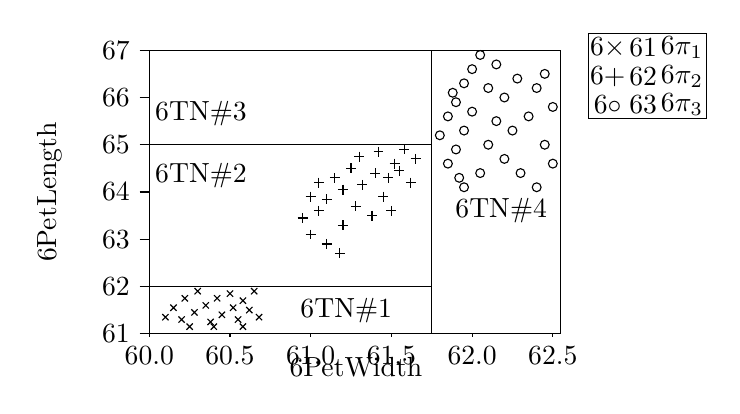
\begin{tikzpicture}[x=2.05cm,y=0.60cm,every node/.style={font=\zihao{6}}]
% 坐标框
\draw (0,1) rectangle (2.55,7);
\draw (1.75,1)--(1.75,7);
\draw (0,2)--(1.75,2);
\draw (0,5)--(1.75,5);
% y 轴刻度
\foreach \yy in {2,3,4,5,6,7} {\draw (-0.06,\yy)--(0,\yy); \node[left] at (-0.06,\yy) {\yy};}
\draw (-0.06,1)--(0,1); \node[left] at (-0.06,1) {1};
% x 轴刻度
\foreach \xx/\lab in {0/0.0,0.5/0.5,1.0/1.0,1.5/1.5,2.0/2.0,2.5/2.5} {\draw (\xx,1)--(\xx,0.93); \node[below] at (\xx,0.93) {\lab};}
% 分组标记
\draw plot[only marks,mark=x,mark size=1.6pt] coordinates{
(0.10,1.35)(0.15,1.55)(0.20,1.30)(0.22,1.75)(0.28,1.45)(0.30,1.90)(0.35,1.60)
(0.38,1.25)(0.42,1.75)(0.45,1.40)(0.50,1.85)(0.52,1.55)(0.55,1.30)(0.58,1.70)
(0.62,1.50)(0.65,1.90)(0.68,1.35)(0.25,1.15)(0.40,1.15)(0.58,1.15)};
\draw plot[only marks,mark=+,mark size=1.8pt] coordinates{
(0.95,3.45)(1.00,3.90)(1.00,3.10)(1.05,3.60)(1.05,4.20)(1.10,2.90)(1.10,3.85)
(1.15,4.30)(1.18,2.70)(1.20,3.30)(1.20,4.05)(1.25,4.50)(1.28,3.70)(1.30,4.75)
(1.32,4.15)(1.38,3.50)(1.40,4.40)(1.42,4.85)(1.45,3.90)(1.48,4.30)(1.52,4.60)
(1.55,4.45)(1.58,4.90)(1.62,4.20)(1.65,4.70)(1.50,3.60)};
\draw plot[only marks,mark=o,mark size=1.6pt] coordinates{
(1.80,5.20)(1.85,5.60)(1.85,4.60)(1.88,6.10)(1.90,4.90)(1.90,5.90)(1.92,4.30)
(1.95,5.30)(1.95,4.10)(1.95,6.30)(2.00,5.70)(2.00,6.60)(2.05,4.40)(2.05,6.90)
(2.10,5.00)(2.10,6.20)(2.15,5.50)(2.15,6.70)(2.20,4.70)(2.20,6.00)(2.25,5.30)
(2.28,6.40)(2.30,4.40)(2.35,5.60)(2.40,6.20)(2.40,4.10)(2.45,5.00)(2.45,6.50)
(2.50,4.60)(2.50,5.80)};
% 区域标注
\node at (0.32,5.65) {TN\#3};
\node at (0.32,4.35) {TN\#2};
\node at (1.22,1.50) {TN\#1};
\node at (2.18,3.60) {TN\#4};
% 轴标题
\node[rotate=90] at (-0.62,4.0) {PetLength};
\node at (1.28,0.30) {PetWidth};
% 图例
\draw (2.72,5.55) rectangle (3.45,7.35);
\node at (2.84,7.05) {$\times$}; \node at (3.06,7.05) {1}; \node at (3.30,7.05) {$\pi_1$};
\node at (2.84,6.45) {$+$};  \node at (3.06,6.45) {2}; \node at (3.30,6.45) {$\pi_2$};
\node at (2.84,5.85) {$\circ$}; \node at (3.06,5.85) {3}; \node at (3.30,5.85) {$\pi_3$};
\end{tikzpicture}
\phantomsection\label{fig:11.19}\mvcap{图 11.19\quad 在花瓣长度—花瓣宽度样本空间的分类树最终结(区域)}
\end{mvfigure}

由于在 TN\#3 中的花大部分属于 $\pi_3$, 这一组中的新项目将归入 $\pi_3$, 即 TN\#3 和 TN\#4 这两组都归入 $\pi_3$ 总体. 我们可以看到, CART 将所有 50 个 $\pi_1$ 品种正确分类, 将 50 个 $\pi_2$ 品种中 47 个正确分类, 将 50 个 $\pi_3$ 品种中 49 个正确分类. 因此 $\mathrm{APER}=\dfrac{4}{150}=0.027$, 这个结果与例 11.12 中用线性判别分析得到的结果大致相对.

CART 方法不依赖总体特征的概率分布, 也不依赖特定的最优性准则. 在实践中, 这种方法需要数百个对象和许多变量. 最后得出的树形图非常复杂, 必须利用主观判断对这棵树进行“修剪”, 使之终止于由若干对象构成的一些组, 而不是所有单个对象. 然后将每个终端组指派给含多数成员的总体, 而一个新对象则可根据其最后的组来分类.

为了实施 CART 分析, 布雷曼、弗里德曼、奥尔森和斯通(Breiman、Friedman、Olsen \& Stone, 见文献[5])开发了一个专用软件. 另外, Loh(见文献[21]和[25])开发了改进的分类树软件, 称为 QUEST\footnote{{\footnotesize 可在 \texttt{www.stat.wisc.edu/\textasciitilde loh/quest.html} 下载.}

\noindent{\footnotesize 可在 \texttt{www.stat.wisc.edu/\textasciitilde loh/cruise.html} 下载.}} 和 CRUISE\textsuperscript{\textcircled{2}}. 他们的程序中采用了若干个明智的分离法则, 通常能产生一棵有很好分离效果的树. CART 在数据挖掘中取得了很大成功(具补充材料 12A).

\mvsub{神经网络}

神经网络(NN)是一种计算机集成的算法过程, 它借助于由相对说比较简单的处理单元(神经元或节)高度连接而成的网络, 将输入转化为所需要的输出. 神经网络以人脑的神经活动为模型. 因此, 神经网络的三个基本特点为: 基本计算单元(神经元或节), 描述各计算单元之间连接状况的网络结构以及用来寻找完成特定工作所需的网络参数(权重)值的训练算法.

神经网络中的计算单元是互相连接的, 因为一个单元的输出可以是另一个单元的输入的一部分. 每个计算单元利用某种预先规定的函数将输入变换为输出, 这种变换在典型的情况下是单调的, 但在其他情况下则是任意的. 这个变换函数依赖于一些其值必须由输入和输出
